\chapter{Introduction}
\label{chap:introduction}

\begin{figure}[ht]
	\hfill
	\begin{minipage}{0.5\textwidth}
		\centering
		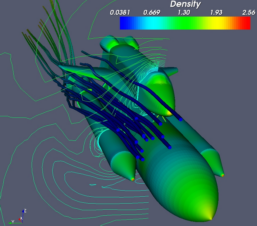
\includegraphics{VTKTextbook-8}\\
		$\downarrow$\\
		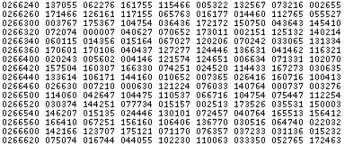
\includegraphics{VTKTextbook-9}
		\caption*{\texttt{Visualization transforms numbers to images.}}
	\end{minipage}
\end{figure}


\firstletter{V}isualization — “2: the act or process of interpreting in
visual terms or of putting into visual form, \emph{Webster’s Ninth New Collegiate Dictionary.}"

\section{What Is Visualization?}
Visualization is a part of our everyday life. From weather maps to the exciting computer graphics of the entertainment industry, examples of visualization abound.
But what is visualization? Informally, visualization is the transformation of data or information into pictures.
Visualization engages the primary human sensory apparatus, vision, as well as the processing power of the human mind.
The result is a simple and effective medium for communicating complex and/or voluminous information

\subsection{Terminology}
Different terminology is used to describe visualization. Scientific visualization is the formal name given to the field in computer science that  ncompasses user interface, data representation and processing algorithms, visual representations, and other sensory presentation such as sound or touch \cite{McCormick87}.
The term data visualization is another phrase used to describe visualization. Data visualization is generally interpreted to be more general than scientific visualization, since it implies treatment of data sources beyond the sciences and engineering. Such data sources include financial, marketing, or business data. In addition, the term data visualization is broad enough to include application of statistical methods and other standard data analysis techniques \cite{Rosenblum94}.
Another recently emerging term is information visualization. 
This field endeavors to visualize abstract information such as hyper-text documents on the World Wide Web, directory/ file structures on a computer, or abstract data structures \cite{InfoVis95}.
A major challenge facing information visualization researchers is to develop coordinate systems, transformation methods, or structures that meaningfully organize and represent data.

Another way to classify visualization technology is to examine the context in which the data exists. If the data is spatial-temporal in nature (up to three spatial coordinates and the time dimension) then typically methods from scientific visualization are used. If the data exists in higher dimensional spaces, or abstract spaces, then methods from information visualization are used.
This distinction is important, because the human perceptual system is highly tuned to space-time relationships.
Data expressed in this coordinate system is inherently understood with little need for explanation. Visualization of abstract data typically requires extensive explanations as to what is being viewed. This is not to say that there is no overlap between scientific and information visualization often the first step in the information visualization process is to project abstract data into the spatial-temporal domain, and then use the methods of scientific visualization to view the results. The projection process can be quite complex, involving methods of statistical graphics, data
mining, and other techniques, or it may be as simple as selecting a lower-dimensional subset of the original data.

In this text we use the term data visualization instead of the more specific terms scientific visualization or information visualization. We feel that scientific visualization is too narrow a description of the field, since visualization techniques have moved beyond the scientific domain and into areas of business, social science, demographics, and information management in general.
We also feel that the term data visualization is broad enough to encompass the term information visualization.

\subsection{Examples of Visualization}
Perhaps the best definition of visualization is offered by example. In many cases visualization is influencing peoples' lives and performing feats that a few years ago would have been unimaginable. A prime example of this is its application to modern medicine.

Computer imaging techniques have become an important diagnostic tool in the practice of modern medicine. These include techniques such as X-ray \emph{Computed Tomography} (CT) and \emph{Magnetic Resonance Imaging} (MRI). These techniques use a sampling or data acquisition process to capture information about the internal anatomy of a living patient. This information is in the form of \emph{slice-planes} or cross-sectional images of a patient, similar to conventional photographic X-rays. CT imaging uses many pencil thin X-rays to acquire the data, while MRI combines large magnetic fields with pulsed radio waves. Sophisticated mathematical techniques are used to reconstruct the slice-planes. Typically, many such closely spaced slices are gathered together into a \emph{volume} of data to complete the study.

As acquired from the imaging system, a slice is a series of numbers representing the attenuation of X-rays (CT) or the relaxation of nuclear spin magnetization (MRI) \cite{Krestel90}. On any given slice these numbers are arranged in a matrix, or regular array. The amount of data is large, so large that it is not possible to understand the data in its raw form. However, by assigning to these numbers a gray scale value, and then displaying the data on a computer screen, structure emerges. This structure results from the interaction of the human visual system with the spatial organization of the data and the gray-scale values we have chosen. What the computer represents as a series of numbers, we see as a cross section through the human body: skin, bone, and muscle. Even more impressive results are possible when we extend these techniques into three dimensions. Image slices can be gathered into volumes and the volumes can be processed to reveal complete anatomical structures. Using modern techniques, we can view the entire brain, skeletal system, and vascular system on a living patient without interventional surgery. Such capability has revolutionized modern medical diagnostics, and will increase in importance as imaging and visualization technology matures.

Another everyday application of visualization is in the entertainment industry. Movie and television producers routinely use computer graphics and visualization to create entire worlds that we could never visit in our physical bodies. In these cases we are visualizing other worlds as we imagine them, or past worlds we suppose existed. It's hard to watch the movies such as \emph{JurassicPark} and \emph{Toy Story} and not gain a deeper appreciation for the awesome Tyrannosaurus Rex, or to be charmed by Toy Story's heroic Buzz Lightyear.

\emph{Morphing} is another popular visualization technique widely used in the entertainment industry. Morphing is a smooth blending of one object into another. One common application is to morph between two faces. Morphing has also been used effectively to illustrate car design changes from one year to the next. While this may seem like an esoteric application, visualization techniques are used routinely to present the daily weather report. The use of isovalue, or contour, lines to display areas of constant temperature, rainfall, and barometric pressure has become a standard tool in the daily weather report.

Many early uses of visualization were in the engineering and scientific community. From its inception the computer has been used as a tool to simulate physical processes such as ballistic trajectories, fluid flow, and structural mechanics. As the size of the computer simulations grew, it became necessary to transform the resulting calculations into pictures. The amount of data overwhelmed the ability of the human to assimilate and understand it. In fact, pictures were so important that early visualizations were created by manually plotting data. Today, we can take advantage of advances in computer graphics and computer hardware. But, whatever the technology, the application of visualization is the same: to display the results of simulations, experiments, measured data, and fantasy; and to use these pictures to communicate, understand, and entertain.

\section{Why Visualize?}

Visualization is a necessary tool to make sense of the flood of information in today's world of computers. Satellites, supercomputers, laser digitizing systems, and digital data acquisition systems acquire, generate, and transmit data at prodigious rates. The Earth-Orbiting Satellite (EOS) transmits terabytes of data every day. Laser scanning systems generate over 500,000 points in a 15 second scan \cite{Waters91}. Supercomputers model weather patterns over the entire earth \cite{Chen93}. In the first four months of 1995, the New York Stock Exchange processed, on average, 333 million transactions per day \cite{NYTimes}. Without visualization, most of this data would sit unseen on computer disks and tapes. Visualization offers some hope that we can extract the important information hidden within the data.

There is another important element to visualization: It takes advantage of the natural abilities of the human vision system. Our vision system is a complex and powerful part of our bodies. We use it and rely on it in almost everything we do. Given the environment in which our ancestors lived, it is not surprising that certain senses developed to help them survive. As we described earlier in the example of a 2D MRI scan, visual representations are easier to work with. Not only do we have strong 2D visual abilities, but also we are adept at integrating different viewpoints and other visual clues into a mental image of a 3D object or plot. This leads to interactive visualization, where we can manipulate our viewpoint. Rotating about the object helps to achieve a better understanding. Likewise, we have a talent for recognizing temporal changes in an image. Given an animation consisting of hundreds of frames, we have an uncanny ability to recognize trends and spot areas of rapid change.

With the introduction of computers and the ability to generate enormous amounts of data, visualization offers the technology to make the best use of our highly developed visual senses. Certainly other technologies such as statistical analysis, artificial intelligence, mathematical filtering, and sampling theory will play a role in large-scale data processing. However, because visualization directly engages the vision system and human brain, it remains an unequaled technology for understanding and communicating data.

Visualization offers significant financial advantages as well. In today's competitive markets, computer simulation teamed with visualization can reduce product cost and improve time to market. A large cost of product design has been the expense and time required to create and test design prototypes. Current design methods strive to eliminate these physical prototypes, and replace them with digital equivalents. This digital prototyping requires the ability to create and manipulate product geometry, simulate the design under a variety of operating conditions, develop manufacturing techniques, demonstrate product maintenance and service procedures, and even train operators on the proper use of the product before it is built. Visualization plays a role in each case. Already CAD systems are used routinely to model product geometry and design manufacturing procedures. Visualization enables us to view the geometry, and see special characteristics such as surface curvature. For instance, analysis techniques such as finite element, finite difference, and boundary element techniques are used to simulate product performance; and visualization is used to view the results. Recently, human ergonomics and anthropometry are being analyzed using computer techniques in combination with visualization \cite{MDHMS}. Three-dimensional graphics and visualization are being used to create training sequences. Often these are incorporated into a hypertext document or World Wide Web (WWW) pages. Another practical use of graphics and visualization has been in-flight simulators. This has been shown to be a significant cost savings as compared to flying real airplanes and is an effective training method.

\section{Imaging, Computer Graphics, and Visualization}
\label{sec:imaging_computer_graphics_visualization}

There is confusion surrounding the difference between imaging, computer graphics, and visualization. We offer these definitions.

\begin{itemize}
  \item  \emph{Imaging}, or image processing, is the study of 2D pictures, or images. This includes techniques to transform (e.g., rotate, scale, shear), extract information from, analyze, and enhance images.
\begin{figure}[ht]
  \centering
  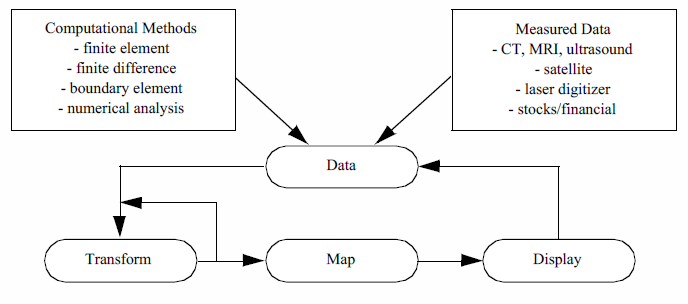
\includegraphics[width=300pt]{Figure1-1}\\
  \caption{The visualization process. Data from various sources is repeatedly transformed to extract, derive, and enhance information. The resulting data is mapped to a graphics system for display.}\label{fig:Figure1-1}
\end{figure}

The resulting data is mapped to a graphics system for display.

  \item  \emph{Computer graphics} is the process of creating images using a computer. This includes both 2D paint-and-draw techniques as well as more sophisticated 3D drawing (or rendering) techniques.

  \item \emph{Visualization} is the process of exploring, transforming, and viewing data as images (or other sensory forms) to gain understanding and insight into the data.
\end{itemize}

Based on these definitions we see that there is overlap between these fields. The output of computer graphics is an image, while the output of visualization is often produced using computer graphics. Sometimes visualization data is in the form of an image, or we wish to visualize object geometry using realistic rendering techniques from computer graphics.

Generally speaking we distinguish visualization from computer graphics and image processing in three ways.

\begin{enumerate}
  \item The dimensionality of data is three dimensions or greater. Many well-known methods are available for data of two dimensions or less; visualization serves best when applied to data of higher dimension.

  \item Visualization concerns itself with data transformation. That is, information is repeatedly created and modified to enhance the meaning of the data.

  \item Visualization is naturally interactive, including the human directly in the process of creating, transforming, and viewing data.
\end{enumerate}

Another perspective is that visualization is an activity that encompasses the process of exploring and understanding data. This includes both imaging and computer graphics as well as data processing and filtering, user interface methodology, computational techniques, and software design. \textbf{Figure \ref{fig:Figure1-1}} depicts this process.

As this figure illustrates we see that the visualization process focuses on data. In the first step data is acquired from some source. Next, the data is transformed by various methods, and then mapped to a form appropriate for presentation to the user. Finally, the data is rendered or displayed, completing the process. Often, the process repeats as the data is better understood or new models are developed. Sometimes the results of the visualization can directly control the generation of the data. This is often referred to as \emph{analysis steering}. Analysis steering is an important goal of visualization because it enhances the interactivity of the overall process.

\section{Origins of Data Visualization}

The origin of visualization as a formal discipline dates to the 1987 NSF report *Visualization in Scientific Computing* \cite{McCormick87}. That report coined the term \emph{scientific visualization}. Since then the field has grown rapidly with major conferences, such as IEEE Visualization, becoming well established. Many large computer graphics conferences, for example ACM SIGGRAPH, devote large portions of their program to visualization technology.

Of course, data visualization technology had existed for many years before the 1987 report referenced \cite{Tufte83}. The first practitioners recognized the value of presenting data as images. Early pictorial data representations were created during the eighteenth century with the arrival of statistical graphics. It was only with the arrival of the digital computer and the development of the field of computer graphics, that visualization became a practicable discipline.

The future of data visualization and graphics appears to be explosive. Just a few decades ago, the field of data visualization did not exist and computer graphics was viewed as an offshoot of the more formal discipline of computer science. As techniques were created and computer power increased, engineers, scientists, and other researchers began to use graphics to understand and communicate data. At the same time, user interface tools were being developed. These forces have now converged to the point where we expect computers to adapt to humans rather than the other way around. As such, computer graphics and data visualization serve as the window into the computer, and more importantly, into the data that computers manipulate. Now, with the visualization window, we can extract information from data and analyze, understand, and manage more complex systems than ever before.

Dr. Fred Brooks, Kenan Professor of Computer Science at the University of North Carolina at Chapel Hill and recipient of the John von Neumann Medal of the IEEE, puts it another way. At the award presentation at the ACM SIGGRAPH '94, Dr. Brooks stated that computer graphics and visualization offer "intelligence amplification" (IA) as compared to artificial intelligence (AI). Besides the deeper philosophical issues surrounding this issue (e.g., human before computer), it is a pragmatic observation. While the long-term goal of AI has been to develop computer systems that could replace humans in certain applications, the lack of real progress in this area has lead some researchers to view the role of computers as amplifiers and assistants to humans. In this view, computer graphics and visualization play a significant role, since arguably the most effective human/ computer interface is visual. Recent gains in computer power and memory are only accelerating this trend, since it is the interface between the human and the computer that often is the obstacle to the effective application of the computer.

\section{Purpose of This Book}

There currently exist texts that define and describe data visualization, many of them using case studies to illustrate techniques and typical applications. Some provide high-level descriptions of algorithms or visualization system architectures. Detailed descriptions are left to academic journals or conference proceedings. What these texts lack is a way to \emph{practice} visualization. Our aim in this text is to go beyond descriptions and provide tools to learn about and apply visualization to your own application area. In short, the purpose of the book is fourfold.

\begin{enumerate}
  \item Describe visualization algorithms and architectures in detail.

  \item Demonstrate the application of data visualization to a broad selection of case studies.

  \item Provide a working architecture and software design for application of data visualization to real-world problems.

  \item Provide effective software tools packaged in a C++ class library. We also provide language bindings for the interpreted languages Tcl, Python, and Java.
\end{enumerate}

Taken together, we refer to the text and software as the \emph{Visualization Toolkit}, or VTK for short. Our hope is that you can use the text to learn about the fundamental concepts of visualization, and then adapt the computer code to your own applications and data.

\section{What This Book Is Not}

The purpose of this book is not to provide a rigorous academic treatise on data visualization. Nor do we intend to include an exhaustive survey of visualization technology. Our goal is to bridge the formal discipline of data visualization with practical application, and to provide a solid technical overview of this emerging technology. In many cases we refer you to the included software to understand implementation details. You may also wish to refer to the appropriate references for further information.

\section{Intended Audience}

Our primary audience is computer users who create, analyze, quantify, and/or process data. We assume a minimal level of programming skill. If you can write simple computer code to import data and know how to run a computer program, you can practice data visualization with the software accompanying this book.

As we wrote this book we also had in mind educators and students of introductory computer graphics and visualization courses. In more advanced courses this text may not be rigorous enough to serve as sole reference. In these instances, this book will serve well as a companion text, and the software is well suited as a foundation for programming projects and class exercises.

Educators and students in other disciplines may also find the text and software to be valuable tools for presenting results. Courses in numerical analysis, computer science, business simulation, chemistry, dynamic systems, and engineering simulations, to name a few, often require large-scale programming projects that create large amounts of data. The software tools provided here are easy to learn and readily adapted to different data sources. Students can incorporate this software into their work to display and analyze their
results.

\section{How to Use This Book}

There are a number of approaches you can take to make effective use of this book. The particular approach depends on your skill level and goals. Three likely paths are as follows:

\emph{Novice}. You're a novice if you lack basic knowledge of graphics, visualization, or object-oriented principles. Start by reading Chapter 2 if you are unfamiliar with object-oriented principles, Chapter 3 if you are unfamiliar with computer graphics, and Chapter 4 if you are unfamiliar with visualization. Continue by reading the application studies in Chapter 12. You can then move on to the CD-ROM and try out some programming examples. Leave the more detailed treatment of algorithms and data representation until you are familiar with the basics and plan to develop your own applications.

\emph{Hacker}. You're a hacker if you are comfortable writing your own code and editing other's. Review the examples in Chapter 3, Chapter 4, and Chapter 12. At this point you will want to acquire the companion software guide to this text ( \emph{The VTK User's Guide} ) or become familiar with the programming resources at \href{https://www.vtk.org/}{VTK}. Then retrieve the examples from the CD-ROM and start practicing.

\emph{Researcher/Educator}. You're a researcher if you develop computer graphics and/or visualization algorithms or if you are actively involved in using and evaluating such systems. You're an educator if you cover aspects of computer graphics and/or visualization within your courses. Start by reading Chapter 2, Chapter 3, and Chapter 4. Select appropriate algorithms from the text and examine the associated source code. If you wish to extend the system, we recommend that you acquire the companion software guide to this text ( \emph{The VTK User's Guide} ) or become familiar with the programming resources at \href{https://www.vtk.org/}{VTK}.

\section{Software Considerations and Example Code}

In writing this book we have attempted to strike a balance between practice and theory. We did not want the book to become a user manual, yet we did want a strong correspondence between algorithmic presentation and software implementation. (Note: *The VTK User's Guide* published by Kitware, Inc. http://www.kitware.com is recommended as a companion text to this book.) As a result of this philosophy, we have adopted the following approach:

\emph{Application versus Design.} The book's focus is the application of visualization techniques to real-world problems. We devote less attention to software design issues. Some of these important design issues include: memory management, deriving new classes, shallow versus deep object copy, single versus multiple inheritance, and interfaces to other graphics libraries. Software issues are covered in the companion text The \emph{VTK User's Guide} published by Kitware, Inc.

\textit{Theory versus Implementation.} Whenever possible, we separate the theory of data visualization from our implementation of it. We felt that the book would serve best as a reference tool if the theory sections were independent of software issues and terminology. Toward the end of each chapter there are separate implementation or example sections that are implementation specific. Earlier sections are implementation free.

\emph{Documentation.} This text contains documentation considered essential to understanding the software architecture, including object diagrams and condensed object descriptions. More extensive documentation of object methods and data members is embedded in the software (in the.h header files) and on CD-ROM or online at \href{https://www.vtk.org/}{VTK}. In particular, the Doxygen generated manual pages contain detailed descriptions of class relationships, methods, and other attributes.

We use a number of conventions in this text. Imported computer code is denoted with a typewriter font, as are external programs and computer files. To avoid conflict with other C++ class libraries, all class names in VTK begin with the " vtk" prefix. Methods are differentiated from variables with the addition of the " ()" postfix. (Other conventions are listed in *VTK User's Guide*.)

All images in this text have been created using the *Visualization Toolkit* software and data found on the included CD-ROM or from the Web site http://www.vtk.org. In addition, every image has source code (sometimes in C++ and sometimes a Tcl script). We decided against using images from other researchers because we wanted you to be able to practice visualization with every example we present. Each computer generated image indicates the originating file. Files ending in.cxx are C++ code, files ending in.tcl are Tcl scripts. Hopefully these examples can serve as a starting point for you to create your own applications.

To find the example code you will want to search in one of three areas. The standard VTK distribution includes an VTK/Examples directory where many well-documented examples are found. The VTK testing directories VTK/Testing, for example, VTK/Graphics/Testing/Tcl, contain some of the example code used in this text. These examples use the data found in the VTKData distribution. Finally, a separate software distribution, the VTKTextbook distribution, contains examples and data that do not exist in the standard VTK distribution. The VTK, VTKData, and VTKTextbook distributions are found on the included CD-ROM and/or on the web site at \href{https://www.vtk.org/}{VTK}.

\section{Chapter-by-Chapter Overview}

\subsection*{Chapter 2: \nameref{chap:object_oriented_design}}

This chapter discusses some of the problems with developing large and/or complex software systems and describes how object-oriented design addresses many of these problems. This chapter defines the key terms used in object-oriented modelling and design and works through a real-world example. The chapter concludes with a brief look at some object-oriented languages and some of the issues associated with object-oriented visualization.

\subsection*{Chapter 3: \nameref{chap:computer_graphics_primer}}

Computer graphics is the means by which our visualizations are created. This chapter covers the fundamental concepts of computer graphics from an application viewpoint. Common graphical entities such as cameras, lights, and geometric primitives are described along with some of the underlying physical equations that govern lighting and image generation. Issues related to currently available graphics hardware are presented, as they affect how and what we choose to render. Methods for interacting with data are introduced.

\subsection*{Chapter 4: \nameref{chap:visualization_pipeline}}

This chapter explains our methodology for transforming raw data into a meaningful representation that can than be rendered by the graphics system. We introduce the notion of a visualization pipeline, which is similar to a data flow diagram from software engineering. The differences between process objects and data objects are covered, as well as how we resolved issues between performance and memory usage. We explain the advantages to a pipeline network topology regarding execution ordering, result caching, and reference counting.

\subsection*{Chapter 5: \nameref{chap:basic_data_representation}}

There are many types of data produced by the variety of fields that apply visualization. This chapter describes the data objects that we use to represent and access such data. A flexible design is introduced where the programmer can interact with most any type of data using one consistent interface. The three high level components of data (structure, cells, and data attributes) are introduced, and their specific subclasses and components are discussed.

\subsection*{Chapter 6: \nameref{chap:fundamental_algorithms}}

Where the preceding chapter deals with data objects, this one introduces process objects. These objects encompass the algorithms that transform and manipulate data. This chapter looks at commonly used techniques for isocontour extraction, scalar generation, color mapping, and vector field display, among others. The emphasis of this chapter is to provide the reader with a basic understanding of the more common and important visualization algorithms.

\subsection*{Chapter 7:  \nameref{chap:advanced_computer_graphics}}

This chapter covers advanced topics in computer graphics. The chapter begins by introducing transparency and texture mapping, two topics important to the main thrust of the chapter: volume rendering. Volume rendering is a powerful technique to see inside of 3D objects, and is used to visualize volumetric data. We conclude the chapter with other advanced topics such as stereoscopic rendering, special camera effects, and 3D widgets.

\subsection*{Chapter 8: \nameref{chap:advanced_data_representation}}

Part of the function of a data object is to store the data. The first chapter on data representation discusses this aspect of data objects. This chapter focuses on basic geometric and topological access methods, and computational operations implemented by the various data objects. The chapter covers such methods as coordinate transformations for data sets, interpolation functions, derivative calculations, topological adjacency operations, and geometric operations such as line intersection and searching.

\subsection*{Chapter 9: \nameref{chap:advanced_algorithms}}

This chapter is a continuation of \emph{Fundamental Algorithms} and covers algorithms that are either more complex or less widely used. Scalar algorithms such as dividing cubes are covered along with vector algorithms such as stream ribbons. A large collection of modelling algorithms is discussed, including triangle strip generation, polygon decimation, feature extraction, and implicit modelling. We conclude with a look at some visualization algorithms that utilize texture mapping.

\subsection*{Chapter 10: \nameref{chap:image_processing}}

While 3D graphics and visualization is the focus of the book, image processing is an important tool for preprocessing and manipulating data. In this chapter we focus on several important image processing algorithms, as well as describe how we use a streaming data representation to process large datasets. 

\subsection*{Chapter 11: \nameref{chap:visuzlization_web}}

The Web is one of the best places to share your visualizations. In this chapter we show you how to write Java-based visualization applications, and how to create VRML (Virtual Reality Modelling Language) data files for inclusion in your own Web content.

\subsection*{Chapter 12: \nameref{chap:applications}}

In this chapter we tie the previous chapters together by working through a series of case studies from a variety of application areas. For each case, we briefly describe the application and what information we expect to obtain through the use of visualization. Then, we walk through the design and resulting source code to demonstrate the use of the tools described earlier in the text.

\section{Legal Considerations}

We make no warranties, expressly or implied, that the computer code contained in this text is free of error or will meet your requirements for any particular application. Do not use this code in any application where coding errors could result in injury to a person or loss of property. If you do use the code in this way, it is at your own risk. The authors and publisher disclaim all liability for direct or consequential damages resulting from your use of this code.

The computer code contained in this text is copyrighted. We grant permission for you to use, copy, and distribute this software for any purpose. However, you may not modify and then redistribute the software. Some of the algorithms presented here are implementations of patented software. If you plan to use this software for commercial purposes, please insure that applicable patent laws are observed.

Some of the data on the CD-ROM may be freely distributed or used (with appropriate acknowledgment). Refer to the local README files or other documentation for details.

Several registered trademarks are used in this text. UNIX is a trademark of UNIX System Laboratories. Sun Workstation and XGL are trademarks of Sun Microsystems, Inc. Microsoft, MS, MS-DOS, and Windows are trademarks of Microsoft Corporation. The X Window System is a trademark of the Massachusetts Institute of Technology. Starbase and HP are trademarks of Hewlett-Packard Inc. Silicon Graphics and OpenGL, are trademarks of Silicon Graphics, Inc. Mac-intosh is a trademark of Apple Computer. RenderMan is a trademark of Pixar.
\section{Bibliographic Notes}

A number of visualization texts are available. The first six texts listed in the reference section are good general references ( \cite{Nielson90}, \cite{Patrikalakis91}, \cite{Brodlie92}, \cite{Wolff93}, \cite{Rosenblum94}, and\cite{Gallagher95} ). Gallagher \cite{Gallagher95} is particularly valuable if you are from a computational background. Wolff and Yaeger \cite{Wolff93} contains many beautiful images and is oriented towards Apple Macintosh users. The text includes a CD-ROM with images and software.

You may also wish to learn more about computer graphics and imaging. Foley and van Dam \cite{FoleyVanDam90} is the basic reference for computer graphics. 

Another recommended text is \cite{BurgerGillies89}. Suggested reference books on computer imaging are \cite{Pavlidis82} and \cite{Wolberg90}.

Two texts by Tufte \cite{Tufte83} \cite{Tufte90} are particularly impressive. Not only are the graphics superbly done, but the fundamental philosophy of data visualization is articulated. He also describes the essence of good and bad visualization techniques.

Another interesting text is available from Siemens, a large company offering medical imaging systems \cite{Krestel90}. This text describes the basic concepts of imaging technology, including MRI and CT. This text is only for those users with a strong mathematical background. A less mathematical
overview of MRI is available from \cite{SmithRanallo89}.

To learn more about programming with Visualization Toolkit, we recommend the text The VTK User’s Guide \cite{UsersGuide}. This text has an extensive example suite as well as descriptions of
the internals of the software. Programming resources including a detailed description of API’s, VTK file formats, and class descriptions are provided.

\printbibliography
